\documentclass[a4paper]{article}
\usepackage{titling}
\usepackage{listings}
\usepackage[english]{babel}
\usepackage[utf8x]{inputenc}
\usepackage{amsmath}
\usepackage{amsfonts}
\usepackage{amssymb}
\usepackage{graphicx}
\usepackage{pseudocode}
\usepackage{algorithm,algpseudocode}

\usepackage{graphicx}
% This package allows to include images
\usepackage{titling}
% This package allows to have a subtitle 
\usepackage{listings}
\usepackage[colorinlistoftodos]{todonotes}
\lstset{%
  basicstyle=\scriptsize\sffamily,%
  commentstyle=\footnotesize\ttfamily,%
  frameround=trBL,
  frame=single,
  breaklines=true,
  showstringspaces=false,
  numbers=left,
  numberstyle=\tiny,
  numbersep=10pt,
  keywordstyle=\bf
}

\title{APP4 Morse code}
\author{PATOTSKAYA Alisa \and PATOTSKAYA Yulia \and REY Ruben \and SID-LAKHDAR Riyane \and PAHEVICH Alexander}

\begin{document}
\maketitle


\tableofcontents



\section{Introduction}
In current report we are observing the solution of the problem, which time complexity will depend on several different input parameters: the size of input string, the size of dictionary and the size of the biggest word in this dictionary. The solutions provided will use dynamic programming for string recognition. 
\section{Polynomial algorithm: first approach}
\subsection{Algorithm description}
In spite of the fact that we have the exponential algorithm, applying it in most of the cases is impossible due to very long time of the computation if parameters $L$ (length of the input string) and $N$ (size of the dictionary) are not very small. Therefore we would like to propose a polynomial algorithm.\\\\
During this algorithm description we will assume that we know an algorithm of finding all substring indexes in a string (for example Knuth–Morris–Pratt). This algorithm must return us all possible position where substring are matching and it works in linear time $O(L)$.\\\\
The idea behind the polynomial algorithm is preprocessing of input stirng and dictionary and applying dynamic programming after. The first thing we want to do is to transform all the dictionary words into Morse code according to our alphabet. From now on we will speak of them as they are written with dots and dashes. Obviously, such transformation can be done in linear time $O(N)$ simply char by char. Input string preprocessing is conducted using substring search algorithm. For every word in dictionary we find all the indexes where it can start and put this information in a matrix which will be used during the algorithm.\\

Matrix $M$ which is obtained during the preprocessing of the input has the structure depicted in the figure \ref{app_matrix.png}. The matrix has $L + 1$ columns and $L$ rows. The column index refers to an index in the input string, the row index refers to size of words. Therefore in $M[i, s]$ we store number of words from the dictionary with size $s$ which the substring searching algorithm has found in the interval $[i, i + s]$. It must be noted that the matrix is triangular as at column $i$ only $L-i$ first rows can be meaningful. The rest of rows refer to words with length more than $L-i$ which can not fit starting from index $i$ in the input string and therefore the substring matching algorithm can not return other value than 0 here. We assumes that the row which refers to words of size $0$ does not exist in the matrix as this row is completely meaningless.\\\\
\begin{figure}[ht!]
	\label{app_matrix.png}
	\center
	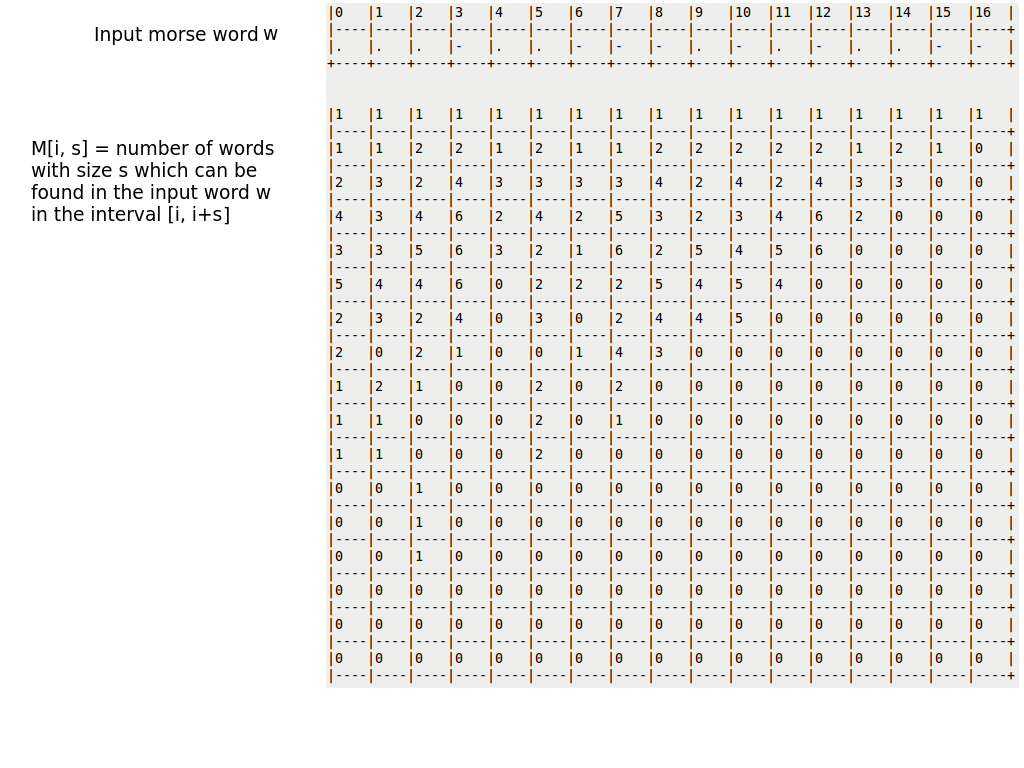
\includegraphics[width=0.8\linewidth]{app_matrix.png}
	\caption{Matrix representing the pre-processed dictionary}
	\label{preprocessing}
\end{figure}

\begin{figure}[ht!]
	\center
	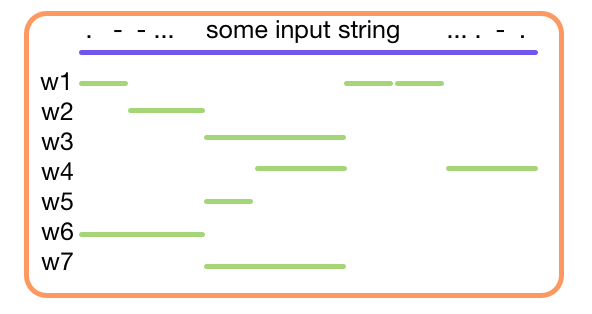
\includegraphics[width=0.8\linewidth]{string_interp.png}
	\caption{String and results of preprocessing}
	\label{preprocessing}
\end{figure}
As soon as we have the results of preprocessing, we can start the algorithm. The idea of the algorithm can be understood from the figure \ref{preprocessing}. The input string is on the top of the figure, all words from dictionary (here 7 of them) are on the left. Green lines next to them correspond to successful matching of this word to corresponding indexes in the input. After we have the green lines, we need to compute the number of combinations of them somehow. Before we introduce the algorithm formula, we would like to define an array $R$ where $R[i]$ contains number of ways how we can decode the sub-string from index $0$ to $i$ of the input. The basic logic of the algorithm is to count possible number of interpretations of sub-string from $0$ to $k$ (which is stored in $R[k]$) as number of interpretations of sub-string from $0$ to $k-1$ ($R[k-1]$) multiplied by number of words found starting from index $k-1$ and of size $1$ ($M[k-1, 1]$) plus $R[k-2] * M[k-2, 2]$ plus $R[k-3] * M[k-3, 3]$ and so on plus number of words found starting from index $0$ and of size $k$ (those which correspond to the full substring). We can write the complete formula:
\begin{equation}
\label{alg_pol_formula}
R[k] = \sum_{j=1}^{k-1}{R[j] * M[j, k-j]} + M[0, k]
\end{equation}
The full pseudo-code can be found in algorithm 3.1. Step with conversion dictionary words to morse code is omitted as it is straightforward: for every latin character we find the morse equivalence and write the corresponding sequence. In the algorithm we first do the input string preprocessing using string matching algorithm and store results in $M$. After it we start to calculate formula \ref{alg_pol_formula} in a simple loop.
\begin{pseudocode}[ruled]{getNumberOfOutputs}{input, dictionary}
 \COMMENT{Polynomial algorithm pseudocode}\\ 
L \GETS length(input)\\
N \GETS length(dictionary)\\
M \GETS \CALL{triangularZeroMatrix}{L + 1, L}\\
\FOR word \textbf{ in } dictionary \DO
	\BEGIN
	arr \GETS \CALL{findSubstrings}{input, word}\\
    \FOR i \textbf{ in } arr \DO
    	M[i, length(word)] \GETS M[i, length(word)] + 1\\
    \END \\
R \GETS [] \\
\FOR i \GETS 0 \TO L \DO 
	R[i] = M[0, i] \\
\FOR i \GETS 0 \TO L - 1 \DO
	\BEGIN
    \IF R[i] == 0 \DO continue \\
    \FOR j \GETS 1 \TO L - i \DO
    	R[i + j] \GETS R[i + j] + R[i] * M[i, j]
    \END \\
\RETURN{R[L]}
\end{pseudocode}
\subsection{Algorithm complexity}
To evaluate the complexity we can just look at the loops. The first loop over the dictionary contains the algorithm of substring matching ($O(L)$) and therefore the whole loop has complexity $O(L*N)$. The next loop of the initialization of $R$ has complexity $O(L)$. The last loop has complexity $O(L^2)$. Therefore the complexity of the algorithm is $O(L*N + L + L^2) = O(L*N + L^2)$ which is perfectly polynomial. We did not mention the conversion of dictionary into Morse code as it has complexity $O(N)$ which is less than $O(L*N + L^2)$.

















\section{Polynomial algorithm: second approach}
\subsection{Data structure}


Let us first encode each word of the given English dictionary into a Morse sequence by applying the encryption function to each character. Each character can be encoded using at most 4 Morse characters (. and -). Therefore, each encoded word's length is bounded by $4 * M$ (where M is the length of the Morse sequence to process).\\

Let put those words into a hashmap data structure W. The keys of this hashmap are the Morse-encoded dictionary words.  The value corresponding to each Morse key word $k_{M}$ is the number of different English word with the same Morse transcription $k_{M}$.\\

For instance, let's suppose a sequence "-....--.-" encodes the following words: "BAC", "BANN", and "DUC". Then W["-....--.-"] = 3. We can build this data structure with a linear complexity O(N * M) where N is the number of words of the dictionary and M the maximum size of such a word.



\subsection{Algorithmic principle}

Let S the Morse sequence of length L that we are trying to decode.   We suppose that a partition P of the string S exists such as $P = [s_{1}, s_{2}, ..., s_{lp}]$. Then the number of ways to decode S following to this partition is given by:
\begin{equation*}
	C(P) = \prod_{i=0}^{lp}{W[s_i]}
\end{equation*}
We can easily notice that the total number of ways to decode the string S equals to the sum of $C(P)$ for all the possible partitions P.\\
We can also notice, that we are only interested in the partitions P such as $\forall s_{i} \in P, s_{i}$ is a key of the hashmap W.  For all the other partitions $P'$ we consider that $C(P') = 0$.\\

Let us consider the last sub-string of any partition P. It should be present in W. In particular, that means there should be a suffix of length t ($1 \leq t \leq 4 * M$), that is present in W. We can notice that there are no suffixes of length $> 4 * M$, that might be present in W.   Thus we are not interested in partitions that have the last sub-string of this length.

Let us calculate F(S): the number of possible partitions of S, such that each of its sub-string is a key of W. We can use dynamic programming approach as follows.\\

\begin{equation}
\label{alg_pol_formula2}
F(S) = \sum_{}{}{ F(S') * W[s]}
\end{equation}

for all prefixes s of S, i.e. S = concat(S', s). Since we don't have any keywords longer than $4 * M$, we can only consider suffixes s of of $length \leq 4 * M$ (all the other input sub-strings will retrieve zero). This formula can be easily proved by induction on length(S), taking F(0) = 1 as a basis for induction.


Since we don't have any keywords longer that 4 * M, we can only consider suffixes s of of $length \leq 4 * M$. This formula can be easily proved by induction on length(S), taking F(0) = 1 as a basis for induction.



\subsection{Algorithm}
1) Build a hashmap W.\\
2) Search the number of sequence interpretations, execute  function below.\\
3) Output F(L) is the total number of sequence interpretations.\\
\begin{pseudocode}[ruled]{getInterpretationsCount}{input, W, M}\\
\COMMENT{Second polynomial algorithm to solve the Morse code problem.}\\
\COMMENT{input - input line in morse code}\\
\COMMENT{W - hashtable built before}\\
\COMMENT{M - length of max english word from dictionary}\\
F \GETS []\\
F[0] \GETS length(input)\\
L \GETS length(input)\\
\FOR i \GETS 1 \TO L \DO
\BEGIN
\FOR suffixLen \GETS 1 \TO min(i, 4 * M)  \DO
	\BEGIN
	factor = W[S.substring(i - suffix_len + 1 .. i)]\\
    F[i] += F[i - suffix_len] * factor
    \END \\
    \END \\
\RETURN{F[L]}
\end{pseudocode}

\subsection{Complexity}
The time complexity of the previous algorithm is clearly the sum of the complexity of building the hash map and the complexity of computing the function F.\\
\begin{itemize}
    \item As we stated above, the time complexity of building the hashtable is $O(N * M)$ where N is the number of words of the dictionary and $M$ the maximum size of such a word (in English).
      The space complexity is $ O(N * (M + M_{morse}) $ where $M_{morse}$ is the maximum size of a morse word (as we said before, $M_{morse} < 4 * M$, thus we could say, that space comlexity is just $ O(N * M)$.
    \item The time complexity of the function F is $O(L * (4 * M)) * W_{lookup complexity}) = O(L * M^2)$, where $W_{lookup complexity}$ is the complexity of getting word from hashtable ($O(M)$, as we calculate hash function from string). Space complexity is O(N).
\end{itemize}
Thus we could see, that we need $ O(N * M)$ time for building hashtable and $O(L * M^2)$ time complexity for finding number of interpretations. However, we could notice that time for building hashtable is just preprocessing time, thus we could do it once and give user numbers of interpretations just with  $O(L * M^2)$ time complexity.





\section{Conclusion}

In the result of current practice session we have developed several algorithm solutions for Morse code interpretation.  We could conclude several things:\\
1) For both cases the time performance directly depends on the size of the dictionary. But the more preferable to use the second algorithm, as the part of time expenses for reading and interpretation the dictionary is spent on cold start, so we could do it just once and on basis of this result find total number of interpretations for user. However, in general we could choice the first algorithm or the second by comparing L, M and N.\\
2) Both solutions use dynamic programming and create correct solution (not approximate).\\
\end{document}






